\documentclass[conference]{IEEEtran}
\IEEEoverridecommandlockouts
% The preceding line is only needed to identify funding in the first footnote. If that is unneeded, please comment it out.
\usepackage{cite}
\usepackage{amsmath,amssymb,amsfonts}
\usepackage{algorithmic}
\usepackage{graphicx}
\usepackage{textcomp}
\usepackage{xcolor}
\def\BibTeX{{\rm B\kern-.05em{\sc i\kern-.025em b}\kern-.08em
    T\kern-.1667em\lower.7ex\hbox{E}\kern-.125emX}}
\begin{document}

\title{Caching in Named Data Networking\\
% {\footnotesize \textsuperscript{*}Note: Sub-titles are not captured in Xplore and
% should not be used}
% \thanks{Identify applicable funding agency here. If none, delete this.}
}

\author{\IEEEauthorblockN{Christoph Langhans}
\IEEEauthorblockA{\textit{University of Lübeck} \\
% \textit{}\\
Lübeck, Germany \\
christoph.langhans@student.uni-luebeck.de}
% \and
% \IEEEauthorblockN{2\textsuperscript{nd} Given Name Surname}
% \IEEEauthorblockA{\textit{dept. name of organization (of Aff.)} \\
% \textit{name of organization (of Aff.)}\\
% City, Country \\
% email address or ORCID}
% \and
% \IEEEauthorblockN{3\textsuperscript{rd} Given Name Surname}
% \IEEEauthorblockA{\textit{dept. name of organization (of Aff.)} \\
% \textit{name of organization (of Aff.)}\\
% City, Country \\
% email address or ORCID}
% \and
% \IEEEauthorblockN{4\textsuperscript{th} Given Name Surname}
% \IEEEauthorblockA{\textit{dept. name of organization (of Aff.)} \\
% \textit{name of organization (of Aff.)}\\
% City, Country \\
% email address or ORCID}
% \and
% \IEEEauthorblockN{5\textsuperscript{th} Given Name Surname}
% \IEEEauthorblockA{\textit{dept. name of organization (of Aff.)} \\
% \textit{name of organization (of Aff.)}\\
% City, Country \\
% email address or ORCID}
% \and
% \IEEEauthorblockN{6\textsuperscript{th} Given Name Surname}
% \IEEEauthorblockA{\textit{dept. name of organization (of Aff.)} \\
% \textit{name of organization (of Aff.)}\\
% City, Country \\
% email address or ORCID}
}

\maketitle

\begin{abstract}
% \textit{Named Data Networking} (NDN) is an enabling technology for the \textit{Internet of Things} (IoT),
% as it provides features like named-based routing and in-network caching. 
% % Caching can help reduce the retrieval delay, and the load on the data producer and to limit the network traffic. 
% % In contrast to common Internet contents IoT data are usually transient and constantly refreshed by the producer. 
% As IoT devices can be limited in energy, storage, and processing capabilities, conventional caching algorithms are not
% suited for IoT domains.

% In this paper, we introduce a novel distributed probabilistic caching strategy that takes the potentially limited
% capabilities of a device into consideration. Also, we compare this solution to traditional 
% caching strategies in terms of data retrieval and network energy efficiency.

\textit{Named Data Networking} (NDN) supports the \textit{Internet of Things} (IoT) with features like named-based routing 
and in-network caching. Traditional caching algorithms are ill-suited for energy, storage, and processing-limited IoT devices. 
This paper presents a novel distributed probabilistic caching strategy considering device limitations. We also compare this solution 
to traditional caching strategies in terms of data retrieval and network energy efficiency.
\end{abstract}

% \begin{IEEEkeywords}
% component, formatting, style, styling, insert
% \end{IEEEkeywords}

\section{Introduction}
% In the Internet of Things (IoT) vision, various wireless devices 
% % with different capabilities in terms of energy, memory, and computational power 
% interact with their physical surrounding environment and the Internet
% in order to support a wide range of context-aware services. Compared to Internet contents, IoT data are typically
% small and transient as new information may be constantly generated by sensors or other IoT devices.

% Due to distinct requirements in IoT systems compared to traditional systems, new network protocols are essential 
% for IoT communications. In recent research, the Information-Centric Networking (ICN) paradigm \cite{b2, b3, b4} is being explored 
% for IoT applications. ICN employs a unique, persistent, and location-independent naming scheme for content packets, 
% eliminating the need for IP addresses in data retrieval. This model offers benefits such as simplified data retrieval 
% and sharing, native mobility support, in-network caching, and content-based security. In particular, in-network caching 
% accelerates data retrieval, reduces network traffic, and minimizes producer-receiver connectivity requirements.

% % In-network caching has been widely investigated in ICN wired networks \cite{b5}. Due to ressource constrained devices,
% % conventional caching strategies are not well suited for the IoT. 
% Since no specific chaching strategy for wireless IoT systems
% is proposed in other works on this topic \cite{b6, b7, b8}, we will introduce one in this paper.

% In this context we define pCASTING, a \textit{probabilistic CAching STrategy for the INternet of thinGs}, which
% considers the data freshness, as well as the energy level and storage capability of a device in the network to adapt
% the caching probability of each node.

In the Internet of Things (IoT), wireless devices interact with their environment and the Internet to support context-aware services. 
As IoT data is smaller and more transient compared to internet content, they require new protocols. Recently, Information-Centric Networking (ICN) has been explored 
for IoT, offering benefits like simplified data retrieval, mobility support, caching, and content-based security \cite{b2, b3, b4}. To address the lack of 
caching strategies for wireless IoT, we introduce pCASTING, a \textit{probabilistic CAching STrategy for the INternet of thinGs} considering data freshness, energy levels, 
and storage capabilities for each network node.

\section{Caching Strategy}

\subsection{Named Data Networking}

% NDN is a content dissemination architecture that uses hierarchical URI-like content names, carried in
% Interest and Data packets. Every NDN Node holds three tables: $(i)$ the Content Store (CS); $(ii)$ the Pending
% Interest Table (PIT); $(iii)$ the Forwarding Information Base (FIB) \cite{b9}.

% The caching system in a node consists of a caching decision strategy and a replacement policy. They specify whether an incoming
% Data packet is cached or which packet should be replaced by a newly cached packet when the CS is full, respectively.

NDN is a content dissemination architecture with hierarchical URI-like content names in Interest and Data packets. 
Each NDN Node has three tables: Content Store (CS), Pending Interest Table (PIT), and Forwarding Information Base (FIB) \cite{b9}. 
The node's caching system comprises a caching decision strategy and a replacement policy, determining whether to cache incoming Data 
packets or which packet to replace in a full Content Store, respectively.

\subsection{pCASTING}

% In our Scenario, a multi-hop wireless network consists of $N$ nodes that are resource-constrained with limited battery energy.
% These nodes can be fixed, e.g., monitoring sensors, or mobile, e.g., smartphones carried by humans. We assume that a set of nodes
% $C = \{1, ..., N_c\}$, with $N_c < N$ act as consumers, while a producer $P$ generates IoT contents with a specific freshness value.
% The rest of the nodes may cache and forward incoming Data packets.

% When a node receives a Data packet with a PIT matching the caching decision is made according to the pCASTING strategy.
% To calculate the caching probability three dynamic attributes related to device and content are taken into account.

In our scenario, a resource-constrained multi-hop wireless network involves $N$ nodes with limited battery energy. Nodes, either fixed 
(e.g., sensors) or mobile (e.g., smartphones), include a set of consumers $C = \{1, ..., N_c\}$, where $N_c < N$ and a producer $P$ generating 
IoT contents with specific freshness. The remaining nodes can cache and forward incoming Data packets. When a node receives a Data packet 
with a matching PIT, the caching decision follows the pCASTING strategy, considering three dynamic attributes related to the device and 
content to calculate the caching probability.

The device-related attributes are \textit{energy level} ($EN$) and \textit{cache occupancy} ($OC$). These values can easily be monitored by the
IoT devices. As a content attribute, we consider the Data \textit{residual freshness} ($FR$). According to NDN, any producer may include in a Data packet a value indicating the freshness $f$ in seconds,
and a timestamp $t_s$ identifying the instant when the information is produced.

We assume that the caching probability is directly (inversely) proportional to each of these parameters. So that for each of the mentioned parameters can be
normalized as $0 \leq EN \leq 1$, $0 \leq OC \leq 1$ where the values $0$ and $1$ mean that the cache or the battery is empty or full, respectively.
The residual freshness can be normalized as $ FR = 1 - \frac{currentTime - t_s}{f}$.
Packets with a negative freshness parameter are considered expired and are not cached at all.


% Concerning the cache occupancy, it is reasonable to assume that the caching probability is inversely proportional to the cache occupancy level.
% This can be represented as parameter $OC$, with $0 \leq OC \leq 1$, where the values $0$ and $1$ mean that the cache is empty or full, respectively.

% As a content attribute, we consider the Data residual freshness. According to NDN, any producer may include in a Data packet a value indicating the freshness $f$ in seconds,
% and a timestamp $t_s$ identifying the instant when the information is produced. We define a normalized freshness parameter $FR$ as:

To define the caching probability of a Data packet, we consider a \textit{Caching Utility Function} $F_u$ that takes into account
all of the normalized parameters above. The function can be written as follows:
$$F_u = \sum_{i = 1}^{N_p} w_i g(x_i)$$

where $N_p$ is the number of parameters and the weights $w_i$ assume a value such that $0 \leq w_i \leq 1$ and $\sum_{i = 1}^{N_p} w_i = 1$.
Therefore the weights express the importance of each parameter in the computing of the utility value.

$F_u$ must assume values in the interval $[0 : 1]$ and gives as a result the node's caching probability.

\begin{figure}[htbp]
    \centerline{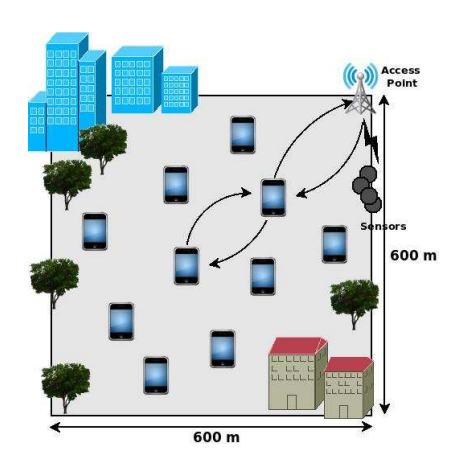
\includegraphics[width=5.5cm]{fig1.png}}
    \caption{Simulation scenario.}
    \label{fig1}
\end{figure}

\subsection{Experiments}


\begin{table}[htbp]
    \caption{Simulation Settings}
    \begin{center}
    \begin{tabular}{c|c|c|}
    \textbf{Category} & \textbf{Paramter}& \textbf{Value} \\
    \hline
    \textbf{Application} & Data packet size & 512 bytes \\
    & Consumer's freshness & rand(1:10) \\
    & Consumer's update period & 1 minute \\
    & $N_d$ & 5 \\
    \hline
    \textbf{NDN} & CS size & 10 packets \\
    & Routing & controlled flooding \cite{b6}, \cite{b15} \\
    & pCASTING & $w_1 = w_2 = w_3 = 1 / 3$ \\
    & & n = 1 \\
    \hline
    \textbf{Access} & Technology & IEEE 802.11g \\
    & Rx Sensitivity & -83 dBm \\
    & Propagation & Rayleigh \\
    \hline
    \textbf{Scenario} & Area Size & 600m x 600m \\
    & Number of movile nodes & 60 \\
    & Mobility Model & pedestrian \cite{b16} \\
    & Number of Consumers & 1-8 \\
    \end{tabular}
    \label{tab1}
    \end{center}
\end{table}

\begin{figure}[htbp]
    \centerline{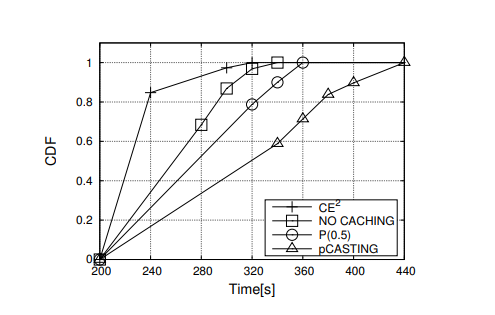
\includegraphics[width=6cm]{fig2.png}}
    \caption{CDF of the discharge time of the forwarding nodes.}
    \label{fig2}
\end{figure}

To evaluate the performance of the proposed pCASTING solution we consider a smart city scenario in Fig. 1 representing an urban 
area of size 600m x 600m. A group of sensors deployed in the city periodically generate data for context-aware services. 
An Access Point offers these services to interested consumers. Each service consists of $N_d$ Data packets. The described scenario and the 
pCASTING solution were implemented in the ndnSIM tool \cite{b10}, the reference simulation platform of the NDN research community deployed 
in ns-3 \cite{b18}. Additional information concerning the simulation settings is listed in Table 1.

In the initial analysis, we aim to assess the energy efficiency of pCASTING while ensuring good performance in terms of retrieval delay and 
collected Data. Consumer nodes start with high initial energy while forwarding nodes start with low initial energy. The simulation concludes 
when all forwarding nodes deplete their energy.

As an energy performance metric, we consider the \textit{cumulative distribution function} (CDF) \textit{of the discharge time of the forwarding nodes}.
As indicators of the dissemination performance, we consider three values as listed in Table 2.

We evaluate pCASTING by comparing it to three reference schemes:
% $(i)$ 
Caching Everything Everywhere ($CE^2$),
%  which caches every incoming packet; 
% $(ii)$ 
a probabilistic scheme denoted as $P(0.5)$,
% caching incoming Data with a fixed probability of $p = 0.5$;
% $(iii)$ 
and a \textit{no caching} scheme.
% , where nodes 
% solely forward incoming packets without utilizing their Content Store (CS). For each caching scheme, the replacement policy employed is LRU.
Results are calculated over ten independent runs and can be examined in Fig. 2 or Table 2, respectively.


\begin{table}[htbp]
    \caption{Data dissemination performance metrics}
    \begin{center}
    \begin{tabular}{c|c|c|c|c|}
    \textbf{Metric} & \textbf{CE$^\text{2}$}& \textbf{No Caching} & \textbf{P(0.5)} & \textbf{pCASTING} \\
    \hline
    \textbf{Cache hit ratio} & $42 \%$ & $0 \%$ & $49 \%$ & $61 \%$ \\
    \hline
    \textbf{Consumers'} & $206$ & $208$ & $217$ & $239$ \\
    \textbf{received data pkts} & & & & \\
    \hline
    \textbf{Data retrieval} & $0.2$ & $0.34$ & $0.18$ & $0.12$ \\
    \textbf{delay[s]} & & & & \\
    \hline
    \end{tabular}
    \label{tab2}
    \end{center}
\end{table}

% In the second experiment, all nodes are fully charged, still the energy consumption is monitored during the
% duration of ten minutes.

% To evaluate the efficiency of the caching strategy from the network point of view, we consider the \textit{number of Interests} and the 
% \textit{number of Data packets} transmitted by the network during the simulation time. To evaluate the efficiency
% from the consumer point of view, we consider the \textit{consumer energy cost}, which is the average ratio
% between the energy spent and the correctly received bits.

\begin{figure}[htbp]
    \centerline{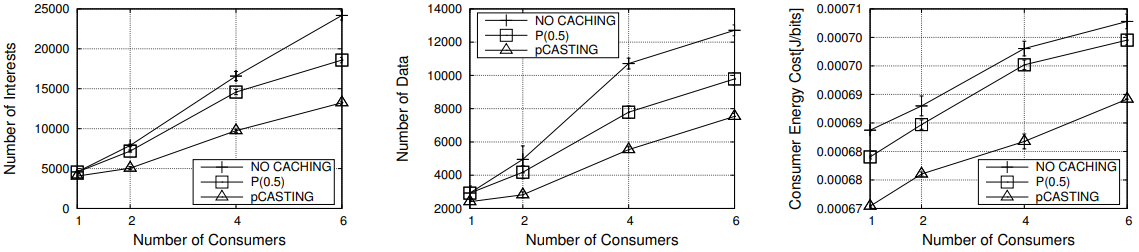
\includegraphics[width=9.5cm]{fig3.png}}
    \caption{Metrics for retrieval performance analysis}
    \label{fig3}
\end{figure}

In the second experiment, fully charged nodes are monitored for energy consumption over ten minutes. Assessing the caching 
strategy's efficiency from the network perspective involves considering the \textit{number of Interests and Data packets} transmitted. 
From the consumer perspective, efficiency is evaluated by examining \textit{consumer energy costs}, calculated as the average ratio of 
energy spent to correctly received bits.

We compare pCASTING against the \textit{no caching} and $P(0.5)$ scheme. Results are averaged over ten independent runs
and can be examined in Fig. 3.


% It can be obtained that pCASTING achieves the best results in all metrics and both experiments due to its
% energy-aware behavior while thanks to the probabilistic caching decision-making, maximizing
% content diversity in the network, increasing the overall performance.

pCASTING outperforms in all metrics and both experiments, showcasing its energy-aware behavior and probabilistic 
caching decision-making. This approach maximizes content diversity, leading to overall improved performance.


\section{Conclusion}
% In this paper, we studied in-network caching in named data wireless IoT networks and proposed a distributed caching
% scheme called pCASTING that adjusts the caching probability
% by considering three main parameters: the battery energy level
% and the cache occupancy of the node, and the Data packet's
% residual freshness. Simulation results proved the effectiveness
% and efficiency of the proposed solution, which is able to reduce
% the energy consumption in the nodes and, at the same time,
% guarantee low content retrieval delays. Since the way we compute the caching probability in pCASTING
% is very simple, it can easily be modified by adding other parameters.

This paper explores in-network caching in named data wireless IoT networks, introducing the distributed caching scheme, pCASTING. 
This scheme adjusts caching probability based on battery energy level, cache occupancy, and Data packet freshness. Simulation results 
confirm the solution's effectiveness, reducing node energy consumption and ensuring low content retrieval delays. The simplicity of pCASTING's 
caching probability computation allows for easy modification by adding additional parameters.

% \section{Prepare Your Paper Before Styling}
% Before you begin to format your paper, first write and save the content as a 
% separate text file. Complete all content and organizational editing before 
% formatting. Please note sections \ref{AA}--\ref{SCM} below for more information on 
% proofreading, spelling and grammar.

% Keep your text and graphic files separate until after the text has been 
% formatted and styled. Do not number text heads---{\LaTeX} will do that 
% for you.

% \subsection{Abbreviations and Acronyms}\label{AA}
% Define abbreviations and acronyms the first time they are used in the text, 
% even after they have been defined in the abstract. Abbreviations such as 
% IEEE, SI, MKS, CGS, ac, dc, and rms do not have to be defined. Do not use 
% abbreviations in the title or heads unless they are unavoidable.

% \subsection{Units}
% \begin{itemize}
% \item Use either SI (MKS) or CGS as primary units. (SI units are encouraged.) English units may be used as secondary units (in parentheses). An exception would be the use of English units as identifiers in trade, such as ``3.5-inch disk drive''.
% \item Avoid combining SI and CGS units, such as current in amperes and magnetic field in oersteds. This often leads to confusion because equations do not balance dimensionally. If you must use mixed units, clearly state the units for each quantity that you use in an equation.
% \item Do not mix complete spellings and abbreviations of units: ``Wb/m\textsuperscript{2}'' or ``webers per square meter'', not ``webers/m\textsuperscript{2}''. Spell out units when they appear in text: ``. . . a few henries'', not ``. . . a few H''.
% \item Use a zero before decimal points: ``0.25'', not ``.25''. Use ``cm\textsuperscript{3}'', not ``cc''.)
% \end{itemize}

% \subsection{Equations}
% Number equations consecutively. To make your 
% equations more compact, you may use the solidus (~/~), the exp function, or 
% appropriate exponents. Italicize Roman symbols for quantities and variables, 
% but not Greek symbols. Use a long dash rather than a hyphen for a minus 
% sign. Punctuate equations with commas or periods when they are part of a 
% sentence, as in:
% \begin{equation}
% a+b=\gamma\label{eq}
% \end{equation}

% Be sure that the 
% symbols in your equation have been defined before or immediately following 
% the equation. Use ``\eqref{eq}'', not ``Eq.~\eqref{eq}'' or ``equation \eqref{eq}'', except at 
% the beginning of a sentence: ``Equation \eqref{eq} is . . .''

% \subsection{\LaTeX-Specific Advice}

% Please use ``soft'' (e.g., \verb|\eqref{Eq}|) cross references instead
% of ``hard'' references (e.g., \verb|(1)|). That will make it possible
% to combine sections, add equations, or change the order of figures or
% citations without having to go through the file line by line.

% Please don't use the \verb|{eqnarray}| equation environment. Use
% \verb|{align}| or \verb|{IEEEeqnarray}| instead. The \verb|{eqnarray}|
% environment leaves unsightly spaces around relation symbols.

% Please note that the \verb|{subequations}| environment in {\LaTeX}
% will increment the main equation counter even when there are no
% equation numbers displayed. If you forget that, you might write an
% article in which the equation numbers skip from (17) to (20), causing
% the copy editors to wonder if you've discovered a new method of
% counting.

% {\BibTeX} does not work by magic. It doesn't get the bibliographic
% data from thin air but from .bib files. If you use {\BibTeX} to produce a
% bibliography you must send the .bib files. 

% {\LaTeX} can't read your mind. If you assign the same label to a
% subsubsection and a table, you might find that Table I has been cross
% referenced as Table IV-B3. 

% {\LaTeX} does not have precognitive abilities. If you put a
% \verb|\label| command before the command that updates the counter it's
% supposed to be using, the label will pick up the last counter to be
% cross referenced instead. In particular, a \verb|\label| command
% should not go before the caption of a figure or a table.

% Do not use \verb|\nonumber| inside the \verb|{array}| environment. It
% will not stop equation numbers inside \verb|{array}| (there won't be
% any anyway) and it might stop a wanted equation number in the
% surrounding equation.

% \subsection{Some Common Mistakes}\label{SCM}
% \begin{itemize}
% \item The word ``data'' is plural, not singular.
% \item The subscript for the permeability of vacuum $\mu_{0}$, and other common scientific constants, is zero with subscript formatting, not a lowercase letter ``o''.
% \item In American English, commas, semicolons, periods, question and exclamation marks are located within quotation marks only when a complete thought or name is cited, such as a title or full quotation. When quotation marks are used, instead of a bold or italic typeface, to highlight a word or phrase, punctuation should appear outside of the quotation marks. A parenthetical phrase or statement at the end of a sentence is punctuated outside of the closing parenthesis (like this). (A parenthetical sentence is punctuated within the parentheses.)
% \item A graph within a graph is an ``inset'', not an ``insert''. The word alternatively is preferred to the word ``alternately'' (unless you really mean something that alternates).
% \item Do not use the word ``essentially'' to mean ``approximately'' or ``effectively''.
% \item In your paper title, if the words ``that uses'' can accurately replace the word ``using'', capitalize the ``u''; if not, keep using lower-cased.
% \item Be aware of the different meanings of the homophones ``affect'' and ``effect'', ``complement'' and ``compliment'', ``discreet'' and ``discrete'', ``principal'' and ``principle''.
% \item Do not confuse ``imply'' and ``infer''.
% \item The prefix ``non'' is not a word; it should be joined to the word it modifies, usually without a hyphen.
% \item There is no period after the ``et'' in the Latin abbreviation ``et al.''.
% \item The abbreviation ``i.e.'' means ``that is'', and the abbreviation ``e.g.'' means ``for example''.
% \end{itemize}
% An excellent style manual for science writers is \cite{b7}.

% \subsection{Authors and Affiliations}
% \textbf{The class file is designed for, but not limited to, six authors.} A 
% minimum of one author is required for all conference articles. Author names 
% should be listed starting from left to right and then moving down to the 
% next line. This is the author sequence that will be used in future citations 
% and by indexing services. Names should not be listed in columns nor group by 
% affiliation. Please keep your affiliations as succinct as possible (for 
% example, do not differentiate among departments of the same organization).

% \subsection{Identify the Headings}
% Headings, or heads, are organizational devices that guide the reader through 
% your paper. There are two types: component heads and text heads.

% Component heads identify the different components of your paper and are not 
% topically subordinate to each other. Examples include Acknowledgments and 
% References and, for these, the correct style to use is ``Heading 5''. Use 
% ``figure caption'' for your Figure captions, and ``table head'' for your 
% table title. Run-in heads, such as ``Abstract'', will require you to apply a 
% style (in this case, italic) in addition to the style provided by the drop 
% down menu to differentiate the head from the text.

% Text heads organize the topics on a relational, hierarchical basis. For 
% example, the paper title is the primary text head because all subsequent 
% material relates and elaborates on this one topic. If there are two or more 
% sub-topics, the next level head (uppercase Roman numerals) should be used 
% and, conversely, if there are not at least two sub-topics, then no subheads 
% should be introduced.

% \subsection{Figures and Tables}
% \paragraph{Positioning Figures and Tables} Place figures and tables at the top and 
% bottom of columns. Avoid placing them in the middle of columns. Large 
% figures and tables may span across both columns. Figure captions should be 
% below the figures; table heads should appear above the tables. Insert 
% figures and tables after they are cited in the text. Use the abbreviation 
% ``Fig.~\ref{fig1}'', even at the beginning of a sentence.

% \begin{table}[htbp]
% \caption{Table Type Styles}
% \begin{center}
% \begin{tabular}{|c|c|c|c|}
% \hline
% \textbf{Table}&\multicolumn{3}{|c|}{\textbf{Table Column Head}} \\
% \cline{2-4} 
% \textbf{Head} & \textbf{\textit{Table column subhead}}& \textbf{\textit{Subhead}}& \textbf{\textit{Subhead}} \\
% \hline
% copy& More table copy$^{\mathrm{a}}$& &  \\
% \hline
% \multicolumn{4}{l}{$^{\mathrm{a}}$Sample of a Table footnote.}
% \end{tabular}
% \label{tab1}
% \end{center}
% \end{table}

% Figure Labels: Use 8 point Times New Roman for Figure labels. Use words 
% rather than symbols or abbreviations when writing Figure axis labels to 
% avoid confusing the reader. As an example, write the quantity 
% ``Magnetization'', or ``Magnetization, M'', not just ``M''. If including 
% units in the label, present them within parentheses. Do not label axes only 
% with units. In the example, write ``Magnetization (A/m)'' or ``Magnetization 
% \{A[m(1)]\}'', not just ``A/m''. Do not label axes with a ratio of 
% quantities and units. For example, write ``Temperature (K)'', not 
% ``Temperature/K''.

% \section*{Acknowledgment}

% The preferred spelling of the word ``acknowledgment'' in America is without 
% an ``e'' after the ``g''. Avoid the stilted expression ``one of us (R. B. 
% G.) thanks $\ldots$''. Instead, try ``R. B. G. thanks$\ldots$''. Put sponsor 
% acknowledgments in the unnumbered footnote on the first page.

% \section*{References}

% Please number citations consecutively within brackets \cite{b1}. The 
% sentence punctuation follows the bracket \cite{b2}. Refer simply to the reference 
% number, as in \cite{b3}---do not use ``Ref. \cite{b3}'' or ``reference \cite{b3}'' except at 
% the beginning of a sentence: ``Reference \cite{b3} was the first $\ldots$''

% Number footnotes separately in superscripts. Place the actual footnote at 
% the bottom of the column in which it was cited. Do not put footnotes in the 
% abstract or reference list. Use letters for table footnotes.

% Unless there are six authors or more give all authors' names; do not use 
% ``et al.''. Papers that have not been published, even if they have been 
% submitted for publication, should be cited as ``unpublished'' \cite{b4}. Papers 
% that have been accepted for publication should be cited as ``in press'' \cite{b5}. 
% Capitalize only the first word in a paper title, except for proper nouns and 
% element symbols.

% For papers published in translation journals, please give the English 
% citation first, followed by the original foreign-language citation \cite{b6}.

\begin{thebibliography}{00}
% \bibitem{b1} J. Gubbi, R. Buyya, S. Marusic, and M. Palaniswami, "Internet of Things (IoT): A Vision, Architectural Elements, and Future Directions," \textit{Elsevier Future Generation Computer Systems}, Volume 29, No. 7, 2013.
\bibitem{b2} B. Ahlgren, C. Dannewitz, C. Imbrenda, D. Kutscher, and B. Ohlman, "A Survey of Information-Centric Networking," \textit{IEEE Communications Magazine}, vol. 50, no. 7, pp. 26-36, 2012.
\bibitem{b3} Y. Zhang \textit{et al.}, "ICN based Architecture for IoT - Requirements and Challenges," in \textit{Internet-Draft}, 2014.
\bibitem{b4} M. Amadeo, C. Campolo, A. Iera, and A. Molinaro, "Named Data Networking for IoT: an Architectural Perspective," in \textit{European Conference on Networks and Communications (EuCNC)}, Bologna, Italy, 2014.
% \bibitem{b5} G. Zhang, Y. Li, and T. Lin, "Caching in Information Centric Networking: a Survey," \textit{Elsevier Computer Networks}, vol. 57, no. 16, 2013.
\bibitem{b6} E. Baccelli et al., "Information Centric Networking in the IoT: Experiments with NDN in the Wild," \textit{ACM ICN}, 2014.
% \bibitem{b7} J. Quevedo, D. Corujo, and R. Aguiar, "Consumer Driven Information Freshness Approach for Content Centric Networking," in \textit{IEEE INFOCOM NOM Workshop}, 2014.
% \bibitem{b8} S. Vural et al., "In-network Caching of Internet-of-Things Data," in \textit{IEEE ICC}, 2014.
\bibitem{b9} L. Zhang et al., "Named Data Networking (NDN) Project," PARC, Tech. Rep. NDN-0001, October 2010.
\bibitem{b10} A. Afanasyev et al., "ndnSIM: NDN simulator for NS-3," University of California, Los Angeles, Tech. Rep. NDN-0005, 2012.
% \bibitem{b11} I. Psaras et al., "Probabilistic In-Network Caching for Information-Centric Networks," in \textit{ACM ICN'12}, 2012.
% \bibitem{b12} S. Tarnoi, K. Suksomboon, W. Kumwilaisak, and Y. Ji, "Performance of Probabilistic Caching and Cache Replacement Policies for Content-Centric Networks," in \textit{IEEE LCN}, 2014.
% \bibitem{b13} W. Shang et al., "Securing Building Management Systems Using Named Data Networking," \textit{IEEE Network}, vol. 3, no. 28, 2014.
% \bibitem{b14} L. Wang et al., "Rapid Traffic Information Dissemination Using Named Data," in \textit{ACM NoM'12}, 2012.
\bibitem{b15} M. Amadeo, C. Campolo, and A. Molinaro, "Forwarding Strategies in Named Data Wireless Ad Hoc Networks: Design and Evaluation," \textit{Elsevier Journal of Network and Computer Applications}, 2014.
\bibitem{b16} I. Rhee, M. Shin, S. Hong, K. Lee, and S. Chong, "On the Levy-walk Nature of Human Mobility," in \textit{IEEE INFOCOM}, 2008.
% \bibitem{b17} "Cisco Aironet 802.11a/b/g Wireless Cardbus Adapter, Data Sheet on line at http://www.cisco.com."
\bibitem{b18} "The network simulator-3 (ns-3), http://www.nsnam.org/."
\end{thebibliography}
\vspace{12pt}
\color{red}
% IEEE conference templates contain guidance text for composing and formatting conference papers. Please ensure that all template text is removed from your conference paper prior to submission to the conference. Failure to remove the template text from your paper may result in your paper not being published.

\end{document}
